\section[Designing Questions]{Designing Questions}

\begin{frame}
  \frametitle{Disclaimer}
  Some examples are inspired by Greg Wilsons book
 \begin{center}
  \sf{Teaching Tech Together} (CRC Press, 2020)
 \end{center}
 Some ideas are based on own experience, some on other sources.
\end{frame}

\subsection{Question Types}

\begin{frame}
  \frametitle{Purposes \ldots}
  Before diving into Question Design, note:
  \begin{itemize}
    \item a question can be asked with a certain aim
    \item different courses ask for different knowledge / skills
    \item $\curvearrowright$ questions need to be designed and choosen with care
  \end{itemize}
\end{frame}

% overview
% background selection

\subsection{Multiple Choice Questions}

\begin{frame}
 \frametitle{Multiple Choice -- When?}

 Multiple Choice Questions (MCQs) are popular when designing e-learning tests \ldots\vspace{-1em}
 \pause
 \newline
 \only<2->{\question{When are they most suitable?}}
 \pause
 Suppose you are teaching children and you give them this MCQ:
 \vspace*{-0.3cm}
 \exercise[Testing Conceptions]{
  What is 37 + 15?
  \begin{enumerate}[a)]
   \item 52  {\color{pdarkgrey}correct}
   \item 42  {\color{pdarkgrey}child did not understand ``carrying''}
   \item 412 {\color{pdarkgrey}child treated every column seperately}
   \item 43  {\color{pdarkgrey}knows she has to carry 1, but to wrong column}
  \end{enumerate}
 }
\end{frame}


\begin{frame}
 \frametitle{Multiple Choice -- When? (continued)}

 The Young-Child question rephrased for newbies to the SLURM batch system:
 \vspace{-1em}
 \exercise[Testing Conceptions about SLURM]{
   Think of a cluster with 20 core nodes. If a job is submitted with the following parameterisation, how many nodes are reserved?\newline
   \texttt{\#SBATCH -n 20}\newline
   \texttt{\#SBATCH -c 2}
   \begin{enumerate}[a)]
    \item 2 {\color{pdarkgrey}correct}
    \item 4 {\color{pdarkgrey}user did correctly multiply, but is not aware of the 20 cores}
    \item 1 {\color{pdarkgrey}user did not multiply by \texttt{-c 2}}
    \item unkown without \texttt{N}-flag {\color{pdarkgrey}user did not understand the concept}
   \end{enumerate}
  }
\end{frame}

\subsection{Beyond MCQ}

\begin{frame}
  \frametitle{What is in the Arsenal?}
  \begin{columns}
   \begin{column}{.5\textwidth}
    MCQs aren't everything:
     \begin{enumerate}
      \item Freetext (if short and explicit)
      \item Filling in blanks (for code; to be implemented)
      \item Parson Problem (can by done as MCQ; shown in a minute)
      \item Tracing (can by done as MCQ; in a minute)
     \end{enumerate}
   \end{column}
   \begin{column}{.5\textwidth}
       \centering
      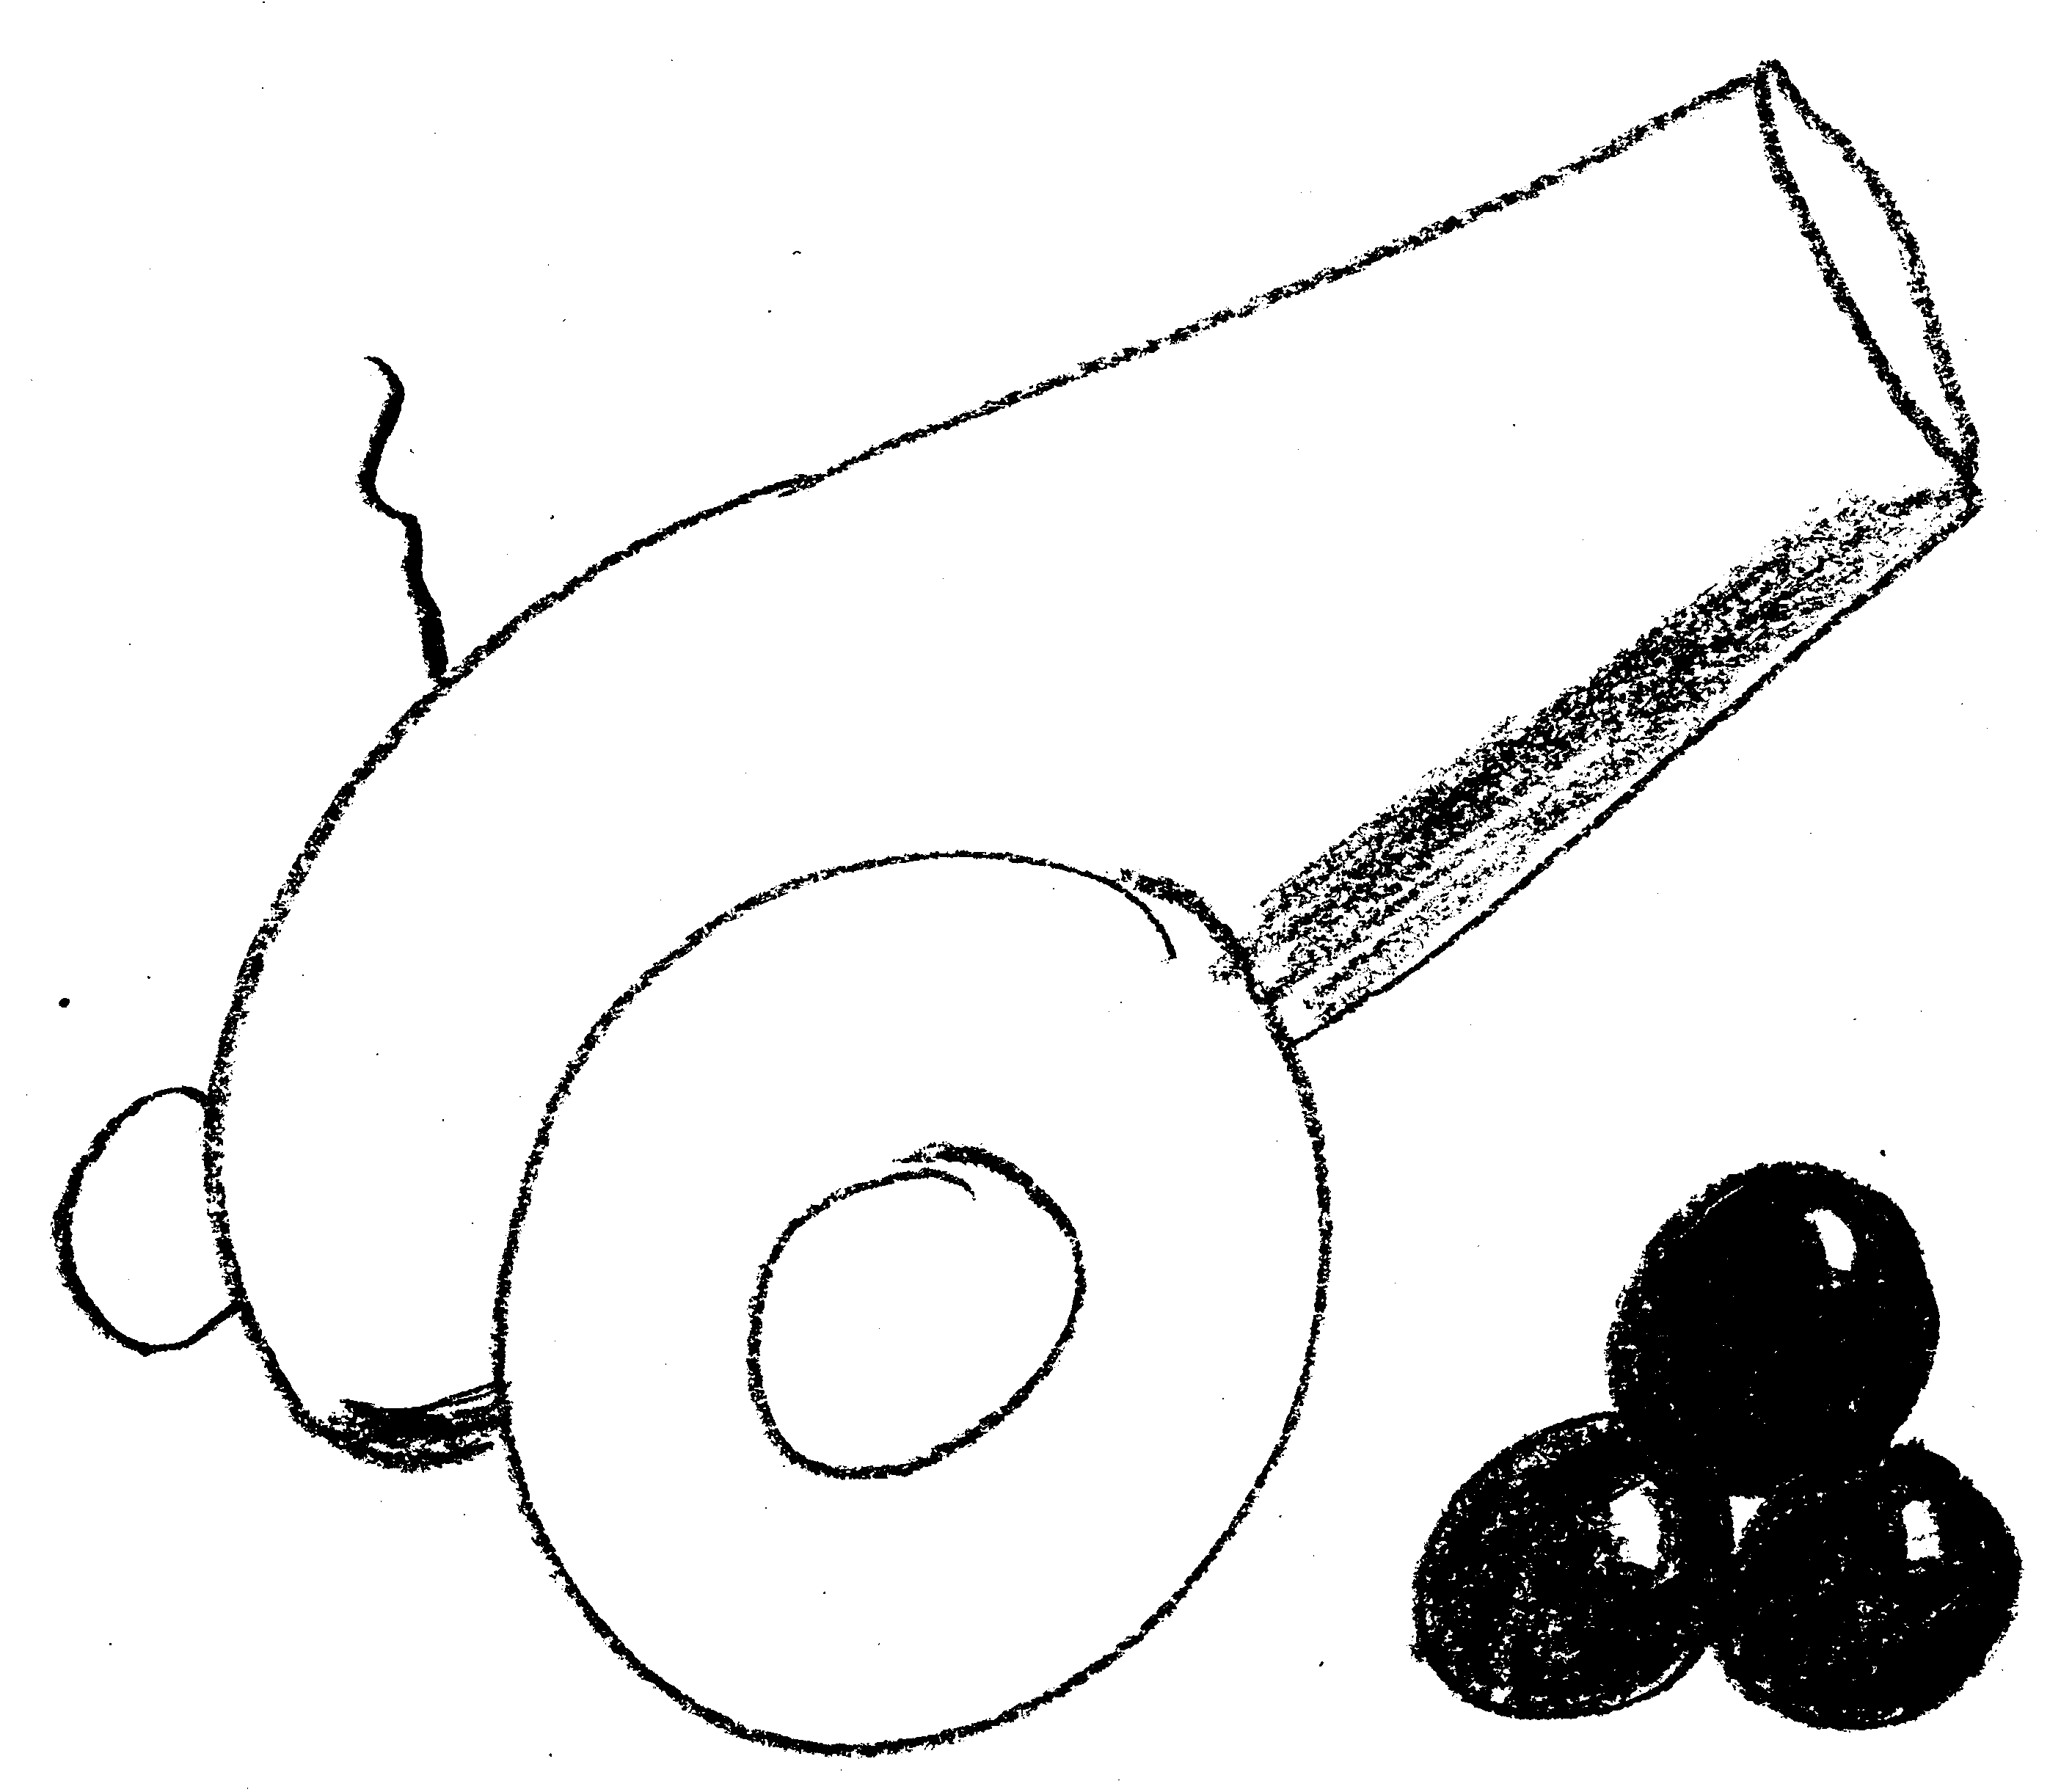
\includegraphics[width=0.6\textwidth]{images/arsenal}
    \end{column}
  \end{columns}
\end{frame}

\begin{frame}<handout:0>
  \frametitle{Freetext}
  Freetext question need to be \emph{very} much restricted to simple words or characters. For example:
  \exercise[Changing Permissions]{
           If a script file 'foo.sh' has the permissions '-rw-r--r--',
           how do make it executable for your group for sharing the script?
           }
  Here, only two possible answers are allowed, in octal or explicit mode.
  \pause
  \hint[Suitability]{This kind is of question is suitable to test actual knowledge. As we can expect only few students to memorize all nifty details, it primarly tests for gained experience and is to be used with great care (not to frequent).}
\end{frame}

\begin{frame}
  \frametitle{Fill in Blanks}
  Filling Blanks is a (technical) variation on Freetext. It is more specific and the \emph{blank screen of horror} issue is avoided, whilst the test might be testing ``vocabulary''. An example:
  \exercise[Bash Operators]{
            Which operator has to be filled in the place of '\_' to print the statement in line 3?\newline
            {\small \bf 1:} \texttt{number=4}\newline
            {\small \bf 2:} \texttt{if [ \$((number {\color{red}\bf\_} 2 )) -eq 0 ]; then}\newline
            {\small \bf 3:} \texttt{~~~~echo "\$number is even"}\newline
            {\small \bf 4:} \texttt{fi}
            }
  \hint{The answer is a single character.}
\end{frame}

\begin{frame}
  \frametitle{Parsons Problems}
  Parsons Problems, too, avoid the \emph{blank screen of horror} problem and also the vocabulary testing. Instead they allow the examinee to concentrate on the control flow.
  \vspace{-.5em}
  \begin{columns}
    \begin{column}{.7\textwidth}
      \exercise[Bash Loop \& Math]{
                Rearrange these lines to sum the values.\newline
                {\small \bf 1:} \texttt{done}\newline
                {\small \bf 2:} \texttt{values=(1 2 3 4)}\newline
                {\small \bf 3:} \texttt{for v in \${values[@]}; do}\newline
                {\small \bf 4:} \texttt{total=\$((total + v))}\newline
                }
    \end{column}
    \begin{column}{.3\textwidth}
      Real tasks can be longer and intricated - allowing test of control flow understanding.
    \end{column}
  \end{columns}
  \vspace{-.5em}
  \hint[Note]{The answer can be a free text, e.\,g.: ``2 3 4 1'', which is easy to parse and check.}
\end{frame}

\subsection{Modyfing the Arsenal}

\begin{frame}<handout:0>[t]
  \frametitle{What else?}
  We could go on \ldots
  \vspace{1em}
  \begin{columns}
    \begin{column}{.7\textwidth}
      \centering
      \begin{tabular}{p{.45\textwidth}p{.55\textwidth}}
         Exercise Type & Technical Implementation\\\hline
         Tracing Code Execution & \only<2->{Freetext or MCQ}\\
         Labelling Diagrams & \only<3->{MCQ}\\
         Fixing Code & \only<4->{Freetext}\\
         etc & \only<5->{Variety of types with minimal technical effort.}
      \end{tabular}
    \end{column}
    \begin{column}{.3\textwidth}
      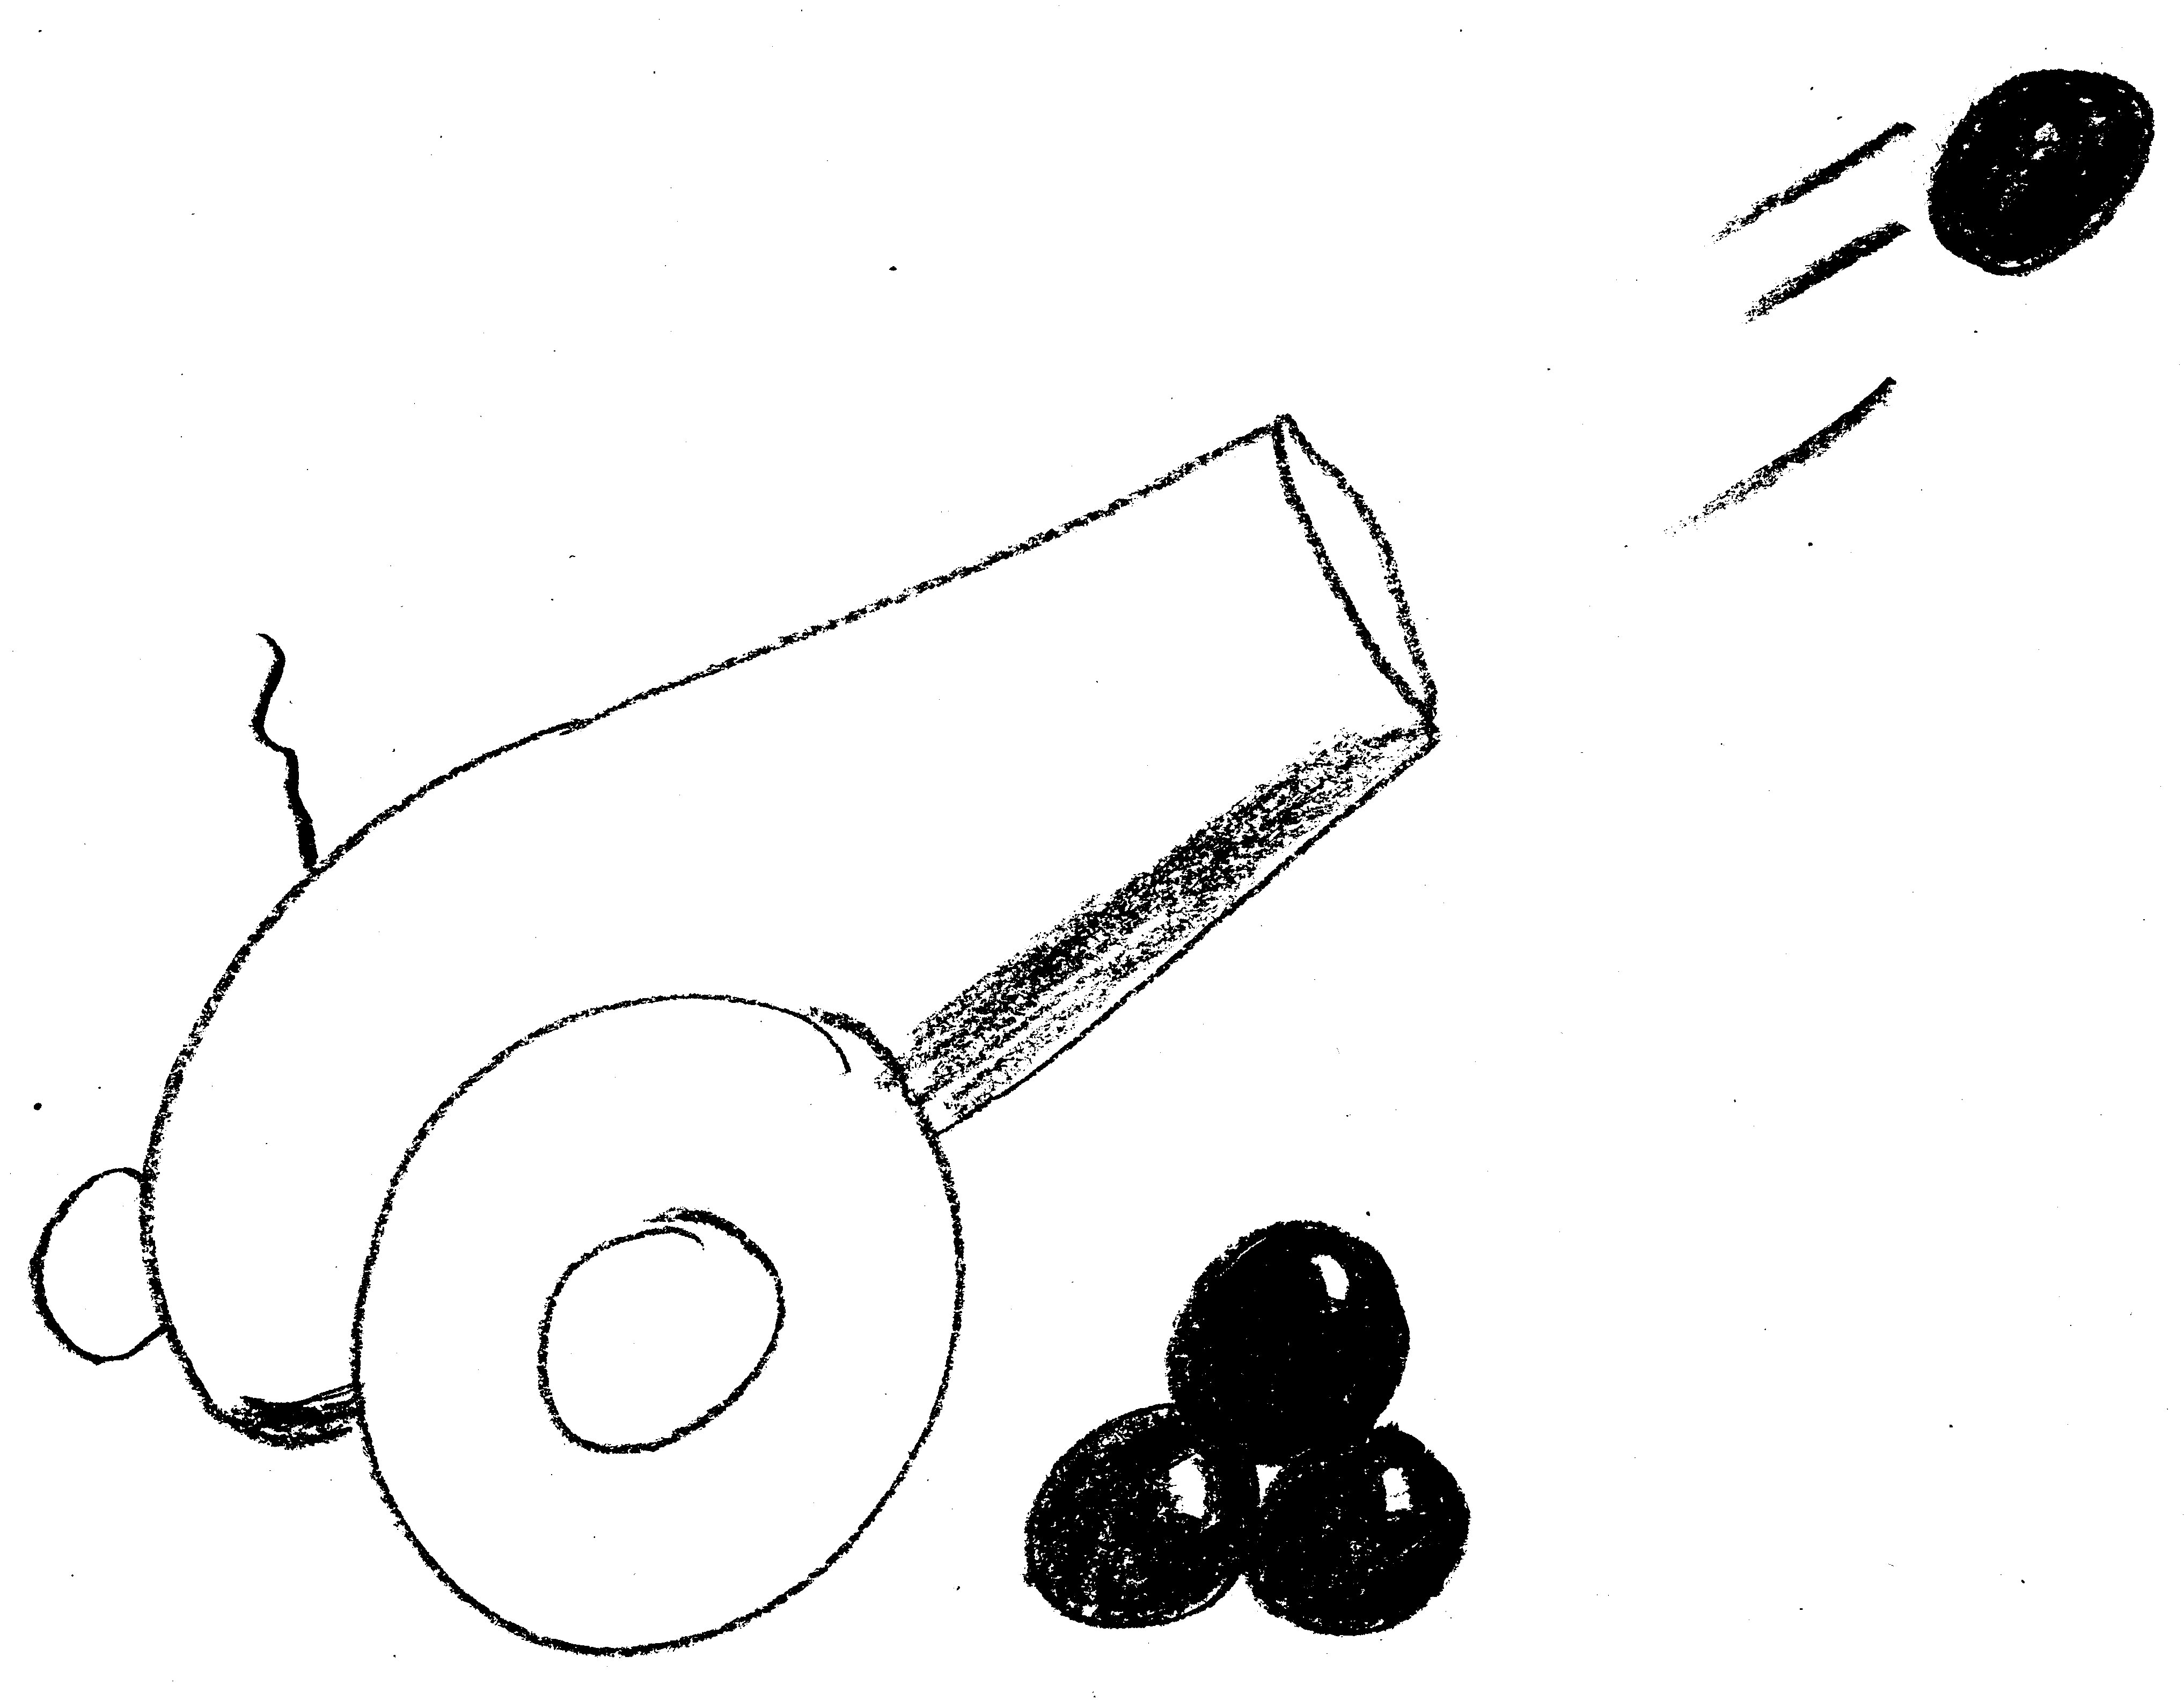
\includegraphics[width=0.6\textwidth]{images/arsenal2}
    \end{column}
   \end{columns}
\end{frame}
